\hypertarget{ux5927ux6a21ux578bux63a8ux7406}{%
\chapter{大模型推理}\label{ux5927ux6a21ux578bux63a8ux7406}}

\hypertarget{ux57faux4e8eux63d0ux793aux7684ux65b9ux6cd5}{%
\section{基于提示的方法}\label{ux57faux4e8eux63d0ux793aux7684ux65b9ux6cd5}}

当下，大模型的推理能力正变得越来越重要。目前模型的推理体现为不断生成token（模型显示正在思考时也在生成token，只不过它们被包裹在特殊的标记中，因此API调用时也会计费），即在``自言自语''中进行显式的逻辑推进。以下是一些基于提示增强模型推理能力的方法。

\hypertarget{ux4e00ux601dux7ef4ux94fechain-of-thought}{%
\subsection{一、思维链（Chain of Thought）}\label{ux4e00ux601dux7ef4ux94fechain-of-thought}}

要求模型逐步思考，将``大问题''拆解为``小步骤''，缩短每一步需要在嵌入空间中``跨越''的距离，进而可以通过每次``预测下一步''实现完整推理。

思维链是大模型推理技术的基石。但其局限性在于，每一步生成只靠先前已生成的内容``从前向后''推断，缺乏从``后续目标''对``先前需要的步骤''的倒推；缺乏自我纠错和反思机制，容易导致错误积累；路径单一，缺乏探索，难以覆盖复杂多样化思考路径。这三种局限性分别对应后面提到的三类方法。

\hypertarget{ux4e8cux4efbux52a1ux89c4ux5212}{%
\subsection{二、任务规划}\label{ux4e8cux4efbux52a1ux89c4ux5212}}

\begin{enumerate}
\def\labelenumi{\arabic{enumi}.}
\tightlist
\item
  规划-执行范式
\end{enumerate}

将推理过程显式地拆分为``规划''和``执行''两个阶段。

规划阶段：模型先不急于计算，而是根据原问题生成一份结构化的计划，列出完成任务所需的关键步骤。这相当于构建了一个全局的指导框架。

执行阶段：模型将计划中的每一步作为单独的输入，逐步生成思维链并得出结果。

优势：通过``先概览、后分步''，减少了中间环节的遗漏和计算错误，特别是在零样本（Zero-shot）场景下，能显著提升模型对未见任务的适应。

\begin{enumerate}
\def\labelenumi{\arabic{enumi}.}
\setcounter{enumi}{1}
\tightlist
\item
  子任务分解（2022）
\end{enumerate}

针对难度超过示例范围的复杂问题（如多步数学推理），可以运用基于``由易到难''的递进思想。将一个复杂问题拆解为一系列子问题，并按难度递增排列，然后依次解决子问题。在解决第 \(k\) 个问题时，会将前 \(k-1\) 个问题的答案作为上下文输入。

这建立了跨步骤的显性依赖关系，利用前序结果辅助当前推理，避免逻辑断裂。

\hypertarget{ux4e09ux52a8ux6001ux8c03ux6574ux4e0eux53cdux601dreflexion2023}{%
\subsection{三、动态调整与反思：Reflexion（2023）}\label{ux4e09ux52a8ux6001ux8c03ux6574ux4e0eux53cdux601dreflexion2023}}

如果说前面的任务规划让模型能``展望未来''，那这里就是让模型``回看过去''，反思自己过去推理轨迹的错误并修正。

架构设计包含三个角色：

\begin{itemize}
\tightlist
\item
  \textbf{行动者（Actor）}：生成行为轨迹 \(\tau\)。
\item
  \textbf{评估者（Evaluator）}：对结果进行打分或判断（如 \(M_e\) 输出布尔信号）。
\item
  \textbf{反思者（Self-Reflector）}：根据失败轨迹和反馈，生成自然语言形式的``反思总结''（\(sr_t\)）并写入记忆。
\end{itemize}

算法流程（基于文档提供的算法伪代码）：

\begin{enumerate}
\def\labelenumi{\arabic{enumi}.}
\tightlist
\item
  初始化策略 \(\pi_\theta\) 和记忆 \(memo\)。
\item
  生成初始轨迹 \(\tau_0\) 并评估。
\item
  循环迭代（当未通过评估且未达最大次数 \(H\)）：

  \begin{itemize}
  \tightlist
  \item
    使用 \(\pi_\theta\) 生成当前轨迹 \(\tau_t\)。
  \item
    使用 \(M_e\) 评估 \(\tau_t\)。
  \item
    使用 \(M_{sr}\) 生成反思 \(sr_t\)。
  \item
    更新记忆：\(mem \leftarrow mem \cup \{sr_t\}\)。
  \item
    下一轮执行时，Actor 将读取 \(mem\) 中的反思信息来修正行为。
  \end{itemize}
\end{enumerate}

本质上，这是把强化学习的过程用语言提示的方式进行了实现。

\hypertarget{ux53c2ux8003ux6587ux732e-123}{%
\subsection{参考文献}\label{ux53c2ux8003ux6587ux732e-123}}

\begin{itemize}
\tightlist
\item
  《动手学大模型智能体》。
\item
  Wei, J., Wang, X., Schuurmans, D., et al.~(2022). \href{https://arxiv.org/abs/2201.11903}{Chain-of-Thought Prompting Elicits Reasoning in Large Language Models}. NeurIPS 2022.
\item
  Shinn, N., Cassano, F., Gopinath, A., Narasimhan, K., \& Yao, S. (2023). \href{https://arxiv.org/abs/2303.11366}{Reflexion: Language Agents with Verbal Reinforcement Learning}. NeurIPS 2023.
\end{itemize}

\clearpage

\hypertarget{ux57faux4e8eux641cux7d22ux7684ux65b9ux6cd5}{%
\section{基于搜索的方法}\label{ux57faux4e8eux641cux7d22ux7684ux65b9ux6cd5}}

前面讲大语言模型时提到，LLM只能输出选择每个token的概率（不管是通过什么方法比如强化学习训练出来的）。``每一步选概率最大的token''这个操作是单步贪婪的，很可能错过全局最优解（如概率第一步0.6第二步0.1和第一步0.4第二步0.9），也因此诞生了Top-K采样、调节温度、集束搜索（每一步保留前k个最好的路径，以便``走着走着发现不好''的时候可以回退）等采样方法。但这些采样方法都没有解决``只看一个token的概率''``只走一条路径''的根本问题，而人类思考难题总是按步骤而非token的，而且对于一个步骤，往往会不同路径都先试一试，然后再选择。

为了克服单一推理路径容易陷入局部最优或单点错误的缺陷，参考集束搜索方法，我们引入基于搜索的推理增强算法，允许智能体探索解空间中的多条路径，以尽可能获得全局最优路径。从数学上来说，线性推理和基于搜索的推理方式可以分别被表达为：

\[
\hat{y}=\arg\max_y P(y\mid x)
\]

\[
\hat{y}=\arg\max_y \sum_{z\in \mathcal{Z}}P(y\mid z,x)P(z\mid x)
\]

其中 \(y\) 代表生成序列，\(z\) 代表并行探索的多个思维路径集合。

两式在数学上相等，但实际意义大不相同。前者是端到端的，如果模型没学好，或者中间逻辑太深，直接拟合 \(P(y\mid x)\)，容易出现误差，而 \(\arg\max\) 操作又容易导致误判（如 \(0.3\) 概率选正确的思路 \(z_1\)，\(0.3\) 概率选正确的思路 \(z_2\)，\(0.4\) 概率选错误的思路 \(z_-\)，结果选最大就朝着错误方向狂奔）。后者中，\(p(z\mid x)\) 即根据问题生成一个合理的解题思路；\(p(y\mid z,x)\) 即根据思路生成答案。显式地建模 \(z\) 能让模型更容易``想清楚''。这相当于把脑子里的模糊直觉（隐层向量）变成了清晰的草稿纸（Token），而且确定 \(z\) 的概率分布可以让我们尽量不受到前述 \(\arg\max\) 随机性的干扰。

另外需要注意的是，搜索算法是``外挂''于模型之外的``采样程序''，就像人类往往需要把完整步骤推演在草稿纸上一样。模型本身（无论是否经过强化学习训练）总是只能生成next token的概率，一般采样方法直接根据这个概率执行动作，基于搜索的方法则先并行在多路径上生成一些内容再选择，最后选择最优作为输出。

下面是一些常见方法：

\hypertarget{ux4e00ux601dux7ef4ux6811}{%
\subsection{一、思维树}\label{ux4e00ux601dux7ef4ux6811}}

通过在主程序中引入树结构，将模型的推理形式化为树状搜索过程。

\begin{enumerate}
\def\labelenumi{\arabic{enumi}.}
\tightlist
\item
  生成：在当前节点（状态）生成多个候选思维分支。注意：一个完整的推理步骤为一个分支，而不是一个token为一个分支（那样树会太宽且太深，稀疏性极高，很难得到有效的价值评估）。提示词会要求模型在一个步骤结束时，生成特定的token作为标识。通过top-k采样只保留几个分支（如5个）。
\end{enumerate}

如果部分任务必须以token为分支做搜索（比如代码补全），可以用模型自身或价值网络先筛选top-k tokens。

\begin{enumerate}
\def\labelenumi{\arabic{enumi}.}
\setcounter{enumi}{1}
\item
  评估：对每个思维节点的潜力，用模型自身或外部函数进行评分，决定保留或剪枝。
\item
  搜索策略：BFS（广度优先）或 DFS（深度优先）。
\end{enumerate}

\hypertarget{ux4e8cux81eaux6211ux4e00ux81f4ux6027}{%
\subsection{二、自我一致性}\label{ux4e8cux81eaux6211ux4e00ux81f4ux6027}}

对同一问题进行多次独立推理，再通过投票机制，把出现频率最高的答案作为最终输出答案。其原理在于，错误推理往往错误原因和路径各不相同，不同错误路径的输出结果较难集中；正确推理路径虽然可能形式不同，但往往会收敛到同一个答案，在概率和采样获得的频率上更有优势。

\hypertarget{ux4e09ux5f15ux5165ux8499ux7279ux5361ux6d1bux6811ux641cux7d22ux7684ux7b97ux6cd5lats2017ux5e74ux66feux7528ux4e8ealphazeroux540eux5f15ux5165llm}{%
\subsection{三、引入蒙特卡洛树搜索的算法（LATS）（2017年曾用于AlphaZero，后引入LLM）}\label{ux4e09ux5f15ux5165ux8499ux7279ux5361ux6d1bux6811ux641cux7d22ux7684ux7b97ux6cd5lats2017ux5e74ux66feux7528ux4e8ealphazeroux540eux5f15ux5165llm}}

\begin{enumerate}
\def\labelenumi{\arabic{enumi}.}
\tightlist
\item
  核心原理（推理时的工作流）
\end{enumerate}

（1）第一阶段：尝试探索

从根节点出发，选择一个最具潜力的子节点进行探索。采用上置信界（UCB）策略，权衡节点的平均价值（该路径过去成功的概率）和访问次数（避免忽略较少探索的路径）。公式通常形式为：

第一阶段：选择（Selection）

从根节点出发，算法需要选择一个最具潜力的子节点进行探索。

\begin{itemize}
\tightlist
\item
  \textbf{策略}：采用上置信界（Upper Confidence Bound, UCT）策略。
\item
  \textbf{原理}：UCT 通过数学公式权衡节点的``平均价值''和``访问次数''。公式通常形式为：
\end{itemize}

\[
UCT=\frac{w_i}{n_i}+C\sqrt{\frac{\ln N}{n_i}}
\]

其中 \(w_i\) 是节点累积价值，\(n_i\) 是节点访问次数，\(N\) 是父节点访问次数，\(C\) 是探索常数。

\begin{itemize}
\tightlist
\item
  \textbf{操作}：算法沿着树向下遍历，直到遇到一个未完全扩展的叶子节点。
\end{itemize}

第二阶段：扩展（Expansion）

在当前选定的节点下，生成新的可能性。

\begin{itemize}
\tightlist
\item
  \textbf{生成器}：由大语言模型（LLM）担任。LLM 根据当前上下文（及历史记忆）生成多个候选操作，例如解题的下一步、一段代码或一个动作。
\item
  \textbf{节点化}：这些生成的候选项构成了搜索树中新的子节点。
\end{itemize}

而实际应用时，我们往往采用改进形式，即PUCT算法：

\[
a_t=\arg\max_a\left(Q(s,a)+U(s,a)\right)
\]

\[
U(s,a)=C_{\mathrm{puct}}\cdot P(s,a)
\frac{\sqrt{\sum_b N(s,b)}}{1+N(s,a)}
\]

Q(s,a)即价值函数，P(s,a)即策略函数pi(s,a)，二者分别由训练好的价值网络和策略网络提供，训练结束后就不再更新。在结合蒙特卡洛树搜索的推理方法中，pi(s,a)不直接作为实际策略输出，而是作为先验概率，反映的是``直觉是往哪里走''，意味着一开始就倾向于认为好的走法而不是乱尝试。N(s,a)代表在s下采取动作a的次数。

（2）第二阶段：扩展路径

遇到一个非推理终点的叶子节点时，根据当前上下文（及历史记忆）生成多个候选操作，例如解题的下一步、一段代码或一个动作（不一定是一个token），这些生成的候选项构成了搜索树中新的子节点。

（3）第三阶段：评估叶子节点的价值

模型不断在当前路径上执行生成的动作，以获得反馈，用于锁定最优路径。如果任务涉及外部环境（如编程），系统会获取编译器或环境的反馈。树的每个节点需要被赋予一个价值分数，来源包括：

运用评估网络：训练一个评估网络（推理时冻结权重），拟合``生成该步骤后，最终得到的奖励期望''。传统的MCTS需要一直随机落子到游戏结束（Rollout），但由于LLM生成的长文本空间极大且成本高昂，对于含有价值网络（Critic）的LLM训练（如PPO算法），可以直接用价值网络中最后一个token的Value近似为评估分数，偏差不大。

模型内评估：LLM自我打分（例如询问：``这条路径逻辑是否通顺？''）。

环境反馈：硬性指标（如测试用例通过率）。

自我反思：LATS将``外部交互''与``长期记忆''融合进了搜索流程。当某次模拟失败时，模型会自动生成一段自然语言的``反思总结''并写入记忆池。后续的扩展步骤中，LLM会读取记忆池中的反思内容。这意味着智能体不会在同一个坑里跌倒两次，而是利用过去的失败修正当前的生成策略。

（4）第四阶段：回传，获得路径上各节点的价值

当前推理路径完成时，在向根节点回退的同时，既更新每个节点的访问次数，也将执行结果（奖励/价值）沿着路径向上逐步回传，直至根节点。每个节点的平均价值，是所有回传到该节点的叶子节点处奖励（如AlphaZero中，叶子节点的奖励为胜利 \(V=1\)，平局 \(V=0\)，失败 \(V=-1\)）的平均值：

对于路径上的每一个节点 \((s_t,a_t)\)，更新公式严格如下：

\begin{enumerate}
\def\labelenumi{\arabic{enumi}.}
\tightlist
\item
  更新总动作价值（累计和）：
\end{enumerate}

\[
W(s_t,a_t)\leftarrow W(s_t,a_t)+V_{\mathrm{leaf}}
\]

\begin{enumerate}
\def\labelenumi{\arabic{enumi}.}
\setcounter{enumi}{1}
\tightlist
\item
  更新访问次数：
\end{enumerate}

\[
N(s_t,a_t)\leftarrow N(s_t,a_t)+1
\]

\begin{enumerate}
\def\labelenumi{\arabic{enumi}.}
\setcounter{enumi}{2}
\tightlist
\item
  计算供第一阶段 UCB/PUCT 使用的平均价值：
\end{enumerate}

\[
Q(s_t,a_t)=\frac{W(s_t,a_t)}{N(s_t,a_t)}
\]

这也意味着，当有探索多条路径经过同一节点时，就会取它们的算术平均值。这使得整棵树能够``记住''哪些分支通向高回报，哪些是死胡同。

这里注意辨析：

在测试阶段，神经网络的权重参数 \(\theta\) 是被冻结（固定）的。

\begin{itemize}
\tightlist
\item
  \textbf{先验概率不变}：对于任何给定的局面 \(s\)，策略网络给出的动作概率 \(P(s,a)\) 是绝对不变的。
\item
  \textbf{单次评估不变}：价值网络对某个叶子节点给出的原始评分 \(v=f_\theta(s_{\mathrm{leaf}})\) 也是绝对不变的。
\end{itemize}

但是，MCTS 搜索树中的 \(Q(s,a)\) 是极其动态的。\(Q(s,a)\) 并不是神经网络直接输出的死数字，而是一个经验平均值，它在测试阶段的几百上千次模拟（Simulations）中随着探索的深入而不断被修正。

\[
Q(s,a)=\frac{W(s,a)}{N(s,a)}
\]

（5）第五阶段：最终决策

当搜索预算（如最大节点数或时间）耗尽后，算法需要输出最终结果。通常选择根节点下访问次数最多的路径作为最优解，因为在MCTS理论中，访问次数多意味着该路径经受住了多次评估且表现优异；也可以以各节点访问次数占比作为它的输出概率进行采样。此外，最终会将关键的反思内容加入长期记忆，为处理下一个任务积累经验。

\begin{enumerate}
\def\labelenumi{\arabic{enumi}.}
\setcounter{enumi}{1}
\tightlist
\item
  AlphaZero
\end{enumerate}

（1）马尔可夫状态的定义

为了保证环境的马尔可夫性，状态 \(s\) 需包括黑白双方棋子的状态，以及当前由谁落子。在训练的过程中，黑白双方均由同一个神经网络控制，每一步的目标都是让己方胜率最大化。需要注意的是，在很多棋类游戏中，未来的状态 \(s_{t+1}\) 和合法动作不仅取决于现在的盘面，还取决于过去发生了什么，因此也需要提取过去几步的盘面作为状态的一部分。以围棋为例：

（2）蒙特卡洛树搜索的展开

蒙特卡洛树搜索（MCTS）的这棵``树''，本质上就是对真实博弈树（Game Tree）的局部展开。在双人交替回合制游戏（如围棋、国际象棋）中，这棵树的层级结构严格对应着现实中的交替回合：

\begin{itemize}
\tightlist
\item
  \textbf{根节点（深度 \(d=0\)）}：轮到``我''行动的当前真实盘面。
\item
  \textbf{子节点（深度 \(d=1\)）}：假设``我''执行了某个动作后，轮到``对手''行动的盘面。
\item
  \textbf{孙子节点（深度 \(d=2\)）}：假设``对手''也执行了动作后，再次轮到``我''行动的盘面。
\end{itemize}

以此类推。

当 MCTS 沿着树不断向下，最终到达一个未被展开的叶子节点 \(s_L\) 时，它会调用神经网络进行评估：

\[
(\mathbf{p},v)=f_\theta(s_L)
\]

这里的价值 \(v\in[-1,1]\) 永远是以``当前节点 \(s_L\) 该落子的一方''为第一视角得出的胜率。

\begin{itemize}
\tightlist
\item
  如果 \(s_L\) 是轮到``我''下，\(v=0.8\) 意味着``我''有极高胜算。
\item
  如果 \(s_L\) 是轮到``对手''下，\(v=0.8\) 意味着``对手''有极高胜算（换言之，``我''快输了）。
\end{itemize}

由于父子节点分属不同阵营，价值 \(v\) 在每次向上一层传递时，必须乘以 \(-1\) 进行符号翻转。

假设在深度 3 的叶子节点（轮到对手下），网络评估 \(v=+0.9\)（对手大优）。

\begin{itemize}
\tightlist
\item
  回传到深度 2（轮到我下）：记录该动作带来的价值为 \(-0.9\)（我很危险）。
\item
  回传到深度 1（轮到对手下）：记录该动作带来的价值为 \(-(-0.9)=+0.9\)（对手很安全）。
\item
  回传到深度 0 根节点（轮到我下）：记录该动作带来的价值为 \(-(+0.9)=-0.9\)（我绝不能走导致这个局面的分支）。
\end{itemize}

无论树搜索当前停留在哪一层，PUCT 都在执行完全相同的最大化公式：

\[
a_t=\arg\max_a\left(
Q(s_t,a)+c_{\mathrm{puct}}\mathbf{p}(a\mid s_t)
\frac{\sqrt{\sum_b N(s_t,b)}}{1+N(s_t,a)}
\right)
\]

\begin{itemize}
\tightlist
\item
  \textbf{当前节点是``我''的回合}：PUCT 会寻找使``我''的 \(Q\) 值最大的动作，同时利用 \(\mathbf{p}\) 和 \(N\) 去探索未知的可能。
\item
  \textbf{当前节点是``对手''的回合}：PUCT 依然在寻找使 \(Q\) 值最大的动作，但因为这里的 \(Q\) 已经站在对手视角计算，所以它实际上是在模拟``对手一定会选择对他最有利、也就是对我最致命的动作''。
\end{itemize}

也就是说，MCTS中模型不仅在考虑``我下了这步棋之后，未来要怎么走''，也在同时预判``我下了这步棋之后，对手会怎么走''。

（3）RL训练方法

树搜索展开（Selection \& Expansion）：从根节点 \(s_t\) 开始，每次利用神经网络 \(f_\theta\) 评估叶子节点，并根据 PUCT 算法选择动作向下搜索，直到达到叶子节点。选择动作的依据不仅考虑胜率 \(Q(s,a)\)，还考虑探索上限 \(U(s,a)\)：

\[
a_t=\arg\max_a\left(
Q(s,a)+c_{\mathrm{puct}}\mathbf{p}(a\mid s)
\frac{\sqrt{\sum_b N(s,b)}}{1+N(s,a)}
\right)
\]

输出改进策略：经过成百上千次模拟后，MCTS 会根据根节点各分支的访问次数 \(N(s_t,a)\) 生成一个更强大的策略分布 \(\pi_t\)：

\[
\pi_t(a\mid s_t)=
\frac{N(s_t,a)^{1/\tau}}
{\sum_b N(s_t,b)^{1/\tau}}
\]

其中 \(\tau\) 是控制探索程度的温度参数。

执行动作与记录：根据 \(\pi_t\) 采样一个动作 \(a_t\) 在真实棋盘上执行。记录下当前状态和 MCTS 改进后的策略 \((s_t,\pi_t)\)。

对局结束：游戏结束时产生最终的真实胜负结果 \(z\in\{-1,0,1\}\)。此时，我们将整局游戏的数据打包为一系列元组：\((s_t,\pi_t,z)\) 存入经验回放池（Replay Buffer）。

在另一个并行的进程中，从经验回放池中随机抽取小批量（Mini-batch）的数据 \((s,\pi,z)\)。使用梯度下降法更新神经网络参数 \(\theta\)，以最小化网络预测值与真实值之间的误差。其损失函数包含两部分（价值均方误差和策略交叉熵）以及 L2 正则化项：

\[
\mathcal{L}(\theta)=(z-v)^2-\boldsymbol{\pi}^{T}\log\mathbf{p}+c\lVert\theta\rVert^2
\]

\begin{itemize}
\tightlist
\item
  \((z-v)^2\)：迫使网络的价值评估 \(v\) 逼近真实的比赛结果 \(z\)（即逼近纳什均衡的真实 Value）。
\item
  \(-\boldsymbol{\pi}^{T}\log\mathbf{p}\)：迫使网络的先验概率 \(\mathbf{p}\) 逼近 MCTS 搜索后得到的更优策略 \(\boldsymbol{\pi}\)（即策略提升过程）。
\end{itemize}

\begin{enumerate}
\def\labelenumi{\arabic{enumi}.}
\setcounter{enumi}{2}
\tightlist
\item
  在大模型中的应用
\end{enumerate}

（1）截断评估

在原始的MCTS算法中，模型一步步推理到末尾才会回传。在长推理中，这极为耗时且计算开销极大。因此我们对于每条路径，生成一层新节点就直接用评估网络打分，即截断式评估。如果发现多个路径分数接近、最终输出不确定性强，才会往后再生成一步。

（2）什么时候需要用蒙特卡洛树搜索？

在强化微调和推理中，可以运用蒙特卡洛树搜索方法进行采样。此时由于采样调整导致实际动作变化，故在参数更新中，对应的优势函数需要调整，以和实际采样策略对应：如运用PPO算法，在计算用于参数更新的优势函数A(s,a)时，Q(s,a)直接取蒙特卡洛树搜索采样得到的路径中，从s出发所有经过a的路径的平均价值（比如生成一步就截断，则某条路径的价值=这一步各个token总实际回报+最后一个token的预期未来回报，这样计算价值时用的就是``实际采样策略下的价值''，比单纯时序差分``只能往后看一个token''偏差更小），V(s)仍为输入s后价值网络的输出值。事实上，这也是后面提到的专家迭代的思想，因为对于搜索到的高价值路径，A(s,a)会增大，从而策略提升以使得a动作概率增大，只不过这里没有用监督学习直接模仿。

在前向推理中，由于搜索会让生成速度更慢，一般只会在慢思考模式、长推理问题中运用该方法（或者其他基于搜索的方法如Tree of Thoughts），在快思考模式、日常问答中则不使用。但即便推理时不显式使用，模型在训练时也学到了这种搜索模式，在逐个token的输出中也会出现``尝试方法A\ldots 发现走不通\ldots 回退\ldots 尝试方法B''这样的思考过程。

由于需要额外的评估网络，该方法算力开销偏大。DeepSeek就没有使用该方法，而是直接将蒙特卡洛思想融入算法中，即GRPO算法。DeepSeek团队认为，只要奖励信号足够清晰（比如数学题答案对不对），迭代次数够多，纯粹的RL（GRPO）就能让模型隐式地学会``尝试-评估-回溯''的过程，并以token流（即状态转移）的形式输出出来。

\hypertarget{ux56dbux76f8ux5173ux6027ux68c0ux7d22}{%
\subsection{四、相关性检索}\label{ux56dbux76f8ux5173ux6027ux68c0ux7d22}}

让模型在推理时回忆相关问题或者对解决问题有用的子问题的思路，就类似于做新题时回想已经做过的类似题或碰到过的二级结论。这和目标导向的强化学习有一点类似，虽然模型不知道怎么去A，但它可能已经学习过怎么去B、C，从中可以类比并合理外推得出去A的方法。这也体现了检索在推理中的重要性。

\hypertarget{ux53c2ux8003ux6587ux732e-124}{%
\subsection{参考文献}\label{ux53c2ux8003ux6587ux732e-124}}

\begin{itemize}
\tightlist
\item
  Yao, S., Yu, D., Zhao, J., et al.~(2023). \href{https://arxiv.org/abs/2305.10601}{Tree of Thoughts: Deliberate Problem Solving with Large Language Models}. NeurIPS 2023.
\item
  Silver, D., Hubert, T., Schrittwieser, J., et al.~(2018). \href{https://www.science.org/doi/10.1126/science.aar6404}{A general reinforcement learning algorithm that masters chess, shogi, and Go through self-play}. Science.
\item
  DeepSeek-AI. (2025). \href{https://arxiv.org/abs/2501.12948}{DeepSeek-R1: Incentivizing Reasoning Capability in LLMs via Reinforcement Learning}. arXiv:2501.12948.
\item
  Zhou, A., Yan, K., Shlapentokh-Rothman, M., Wang, H., \& Wang, Y.-X. (2023). \href{https://arxiv.org/abs/2310.04406}{Language Agent Tree Search Unifies Reasoning, Acting, and Planning in Language Models}. ICML 2024.
\end{itemize}

\clearpage

\hypertarget{alphaevolve}{%
\section{AlphaEvolve}\label{alphaevolve}}

\hypertarget{ux4e00ux6838ux5fc3ux601dux60f3-10}{%
\subsection{一、核心思想}\label{ux4e00ux6838ux5fc3ux601dux60f3-10}}

在一些大模型将LLM与搜索算法结合的同时，AlphaEvolve则将LLM与类似遗传算法的优化方式结合，以既有代码库为上下文，用LLM生成大量程序，然后用验证器验证，留下得分更优的代码存入代码库，从而在代码库（上下文）中不断迭代提升。

AlphaEvolve不再依赖人工设计的变异算子（如传统的遗传算法），而是利用LLM丰富的世界知识和编程能力来充当``智能变异算子''，对代码进行有意义的修改。这也可以视为一种通过在权重不变的前提下，更新上下文来实现策略提升的算法。

\hypertarget{ux4e8cux5de5ux4f5cux6d41-1}{%
\subsection{二、工作流}\label{ux4e8cux5de5ux4f5cux6d41-1}}

\begin{enumerate}
\def\labelenumi{\arabic{enumi}.}
\item
  初始化：人类科学家定义问题，提供初始代码，并标记出需要进化的代码块。初始化一个动态数据库模拟种群，存储不同代码。提供一个自动评估函数，用于给生成的代码打分。
\item
  采样与提示构建：从数据库中采样出一个``父本程序''以及若干``灵感程序''。Prompt Sampler 将这些代码、过去的优异解、以及系统指令组装成一个包含丰富上下文的提示词发送给LLM。
\item
  LLM生成与变异：根据提示词，提出对父本程序的修改。输出通常是Diff格式（即差异补丁），只输出代码的修改内容，再由自动化脚本转换为修改后子程序的完整文件。
\item
  代码执行与评估：新程序被发送到评估器中实际运行，运行用户定义的evaluate函数，计算出一个或多个指标（如准确率、速度、数学属性等）。对于耗时的任务，系统支持级联评估：先用小规模测试快速筛选，通过后再进行大规模测试。
\item
  数据库更新：如果新程序的表现优异，它会被存入程序数据库。
\end{enumerate}

\hypertarget{ux4e09ux8fd0ux7528ux573aux666f}{%
\subsection{三、运用场景}\label{ux4e09ux8fd0ux7528ux573aux666f}}

以上是以代码为例，但实际上，作为一种优化算法（无非是把算子换成了LLM），它可以进化不同层级的对象，如直接优化字符串或数值、编写一个生成解的函数、进化用于搜索答案的算法等。其中进化算法这种``工具性目标''通常比直接搜索更有效。

当然，AlphaEvolve还可以进化提示词本身。它将LLM的系统指令和上下文也视为可以优化的对象，在另一个并行的进化过程中不断改进``如何向LLM提问''，从而获得更好的代码生成效果。

\hypertarget{ux56dbux5173ux952eux6280ux672fux7ec4ux4ef6ux548cux7b56ux7565}{%
\subsection{四、关键技术组件和策略}\label{ux56dbux5173ux952eux6280ux672fux7ec4ux4ef6ux548cux7b56ux7565}}

\hypertarget{ux4e00llmux96c6ux6210ux7b56ux7565}{%
\subsubsection{（一）LLM集成策略}\label{ux4e00llmux96c6ux6210ux7b56ux7565}}

Flash：速度快、延迟低。用于生成大量的候选代码，快速探索搜索空间。

Pro：能力更强。用于相对低频率地提供高质量、深度的修改代码，帮助进化过程突破瓶颈，产生``质的飞跃''。

Flash和Pro生成的代码均被发送到评估器，按客观评估得分决定是否保留。

\hypertarget{ux4e8cux5f02ux6b65ux5e76ux53d1}{%
\subsubsection{（二）异步并发}\label{ux4e8cux5f02ux6b65ux5e76ux53d1}}

系统采用asyncio实现异步并发。Controller、LLM Samplers和Evaluators是解耦的，最大化了吞吐量。即使单个评估需要数小时（如训练模型），整个进化过程也不会阻塞。

\hypertarget{ux4e09ux6570ux636eux5e93ux7ef4ux62a4}{%
\subsubsection{（三）数据库维护}\label{ux4e09ux6570ux636eux5e93ux7ef4ux62a4}}

运用MAP-Elites类算法，将解空间划分为不同的``生态位''。

\begin{enumerate}
\def\labelenumi{\arabic{enumi}.}
\tightlist
\item
  ``生态位''的划分方式：根据多个评估指标
\end{enumerate}

（1）用户提供的evaluate函数：它会返回一个包含多个标量值的字典，其中的标量值（如准确率、运行速度、内存占用、代码长度等）构成了包含多重可优化指标的特征空间，根据这些指标的不同组合来划分生态位。如一个生态位可能存放``速度极快但代码较长''的程序，另一个生态位可能存放``速度稍慢但内存占用极低''的程序。

AlphaEvolve明确提到，优化多个指标（即使只关心其中一个）有助于发现具有不同结构或逻辑的程序。也就是说，这是一种可以优化多个变量的算法。

（2）LLM评分：LLM可以对代码的简洁性、可读性或其他风格特征进行打分，这些分数会被添加到评估结果字典中，成为定义生态位的额外维度。例如，一个``逻辑非常清晰简洁''的代码即便性能稍弱，也可能因为占据了``高可读性''这一生态位而被保留下来。

\begin{enumerate}
\def\labelenumi{\arabic{enumi}.}
\setcounter{enumi}{1}
\tightlist
\item
  选择每轮留下的解的原则
\end{enumerate}

利用：当生成一个新的解时，如果它在某个特定的生态位中表现优于现有的解，它就会覆盖旧的解；如果不如现有解，则会被丢弃。总之，就是把表现最优的解留下来。

探索：对于结构独特、处于和现有解均不同的生态位的解，将其留下来，以保证数据库的多样性。

以上考虑到数据库的主要目标是优化地重现之前探索过的想法，以便在未来的数代进化中使用，倾向于保留那些有价值的、高质量的或具有独特性的``精英''代码，同时尽可能保留多样性以免过早收敛到局部最优，而不是无限期地存储所有生成的历史垃圾代码。

\begin{enumerate}
\def\labelenumi{\arabic{enumi}.}
\setcounter{enumi}{2}
\tightlist
\item
  岛屿模型的物理隔离
\end{enumerate}

除了基于特征的生态位，AlphaEvolve 还结合了岛屿模型，将种群物理分割成不同的``岛屿''（子种群），人为地创造了隔离的生态环境。即使两个程序在指标上相似，如果它们属于不同的``岛屿''，它们也可以共存而不被互相淘汰。这强制保持了遗传来源的多样性。

\hypertarget{ux56dbux7236ux672cux7a0bux5e8fux548cux7075ux611fux7a0bux5e8fux7684ux9009ux53d6}{%
\subsubsection{（四）父本程序和灵感程序的选取}\label{ux56dbux7236ux672cux7a0bux5e8fux548cux7075ux611fux7a0bux5e8fux7684ux9009ux53d6}}

\begin{enumerate}
\def\labelenumi{\arabic{enumi}.}
\tightlist
\item
  父本程序（Parent Program）的选取
\end{enumerate}

父本是被LLM直接修改的基础代码。选取策略旨在平衡利用与探索，相对而言利用更多（因为还有灵感作为探索机制）。

利用：系统会高频采样那些当前评分最高、表现最好的程序，让LLM在它们的基础上进行微调，试图进一步推高分数。

探索：为了防止陷入局部最优，系统也会采样那些``表现尚可但结构独特''``处于不同生态位''的程序。

岛屿模型的轮转：如果使用了岛屿模型，父本可能来自不同的``岛屿''（即独立的进化子种群），这有助于保持种群的遗传多样性，防止所有父本都趋同。

\begin{enumerate}
\def\labelenumi{\arabic{enumi}.}
\setcounter{enumi}{1}
\tightlist
\item
  灵感程序（Inspirations）的选取
\end{enumerate}

灵感程序是作为Prompt中的上下文示例展示给LLM的，它们不会被直接修改，而是作为参考。灵感程序选取的一个关键原则是多样性。特别是在多目标优化（例如同时优化速度和内存）的场景下，系统会选取在不同指标上表现优异的程序，如一个运行速度极快但代码较长的程序，和一个代码极简但速度稍慢的程序，同时放入Prompt作为灵感，让LLM生成结合了各家之长的新颖解，或者通过观察不同解法的差异获得``灵感'' 。

\begin{enumerate}
\def\labelenumi{\arabic{enumi}.}
\setcounter{enumi}{2}
\tightlist
\item
  技术背景
\end{enumerate}

AlphaEvolve 不只是随机抽取旧代码，其核心在于In-Context Learning（上下文学习）与进化策略的结合：父本决定了进化的起点；灵感决定了进化的方向指引。通过精心挑选``灵感''，系统实际上是在构建一个动态的Prompt，利用LLM强大的上下文理解能力，将数据库中蕴含的隐性知识（比如某种特定的编程模式在当前任务中很有效）显式地传递给LLM，从而提高生成高质量Diff的概率。

\hypertarget{ux53c2ux8003ux6587ux732e-125}{%
\subsection{参考文献}\label{ux53c2ux8003ux6587ux732e-125}}

\begin{itemize}
\tightlist
\item
  Novikov, A., Vu, N., Eisenberger, M., et al.~(2025). \href{https://arxiv.org/abs/2506.13131}{AlphaEvolve: A coding agent for scientific and algorithmic discovery}. arXiv:2506.13131.
\end{itemize}

\clearpage

\hypertarget{ux591aux8f6eux63a8ux7406ux548cux5e76ux884cux63a8ux7406ux8bbaux6587}{%
\section{多轮推理和并行推理（论文）}\label{ux591aux8f6eux63a8ux7406ux548cux5e76ux884cux63a8ux7406ux8bbaux6587}}

\begin{quote}
本文是论文阅读笔记，内容代表对应论文方法或作者理解，不应直接视为领域共识或工程最佳实践。
\end{quote}

在基准测试中，模型的Pass@K往往明显高于Pass@1。多轮推理和并行推理本质是用推理时的计算量（Test-time Compute）来换取更高的智能表现。虽然这可能导致首字延迟略微增加（通常几秒到几分钟），但对于高难度推理和Agent任务，准确率有质的飞跃。

\hypertarget{ux4e00ux591aux8f6eux63a8ux7406}{%
\subsection{一、多轮推理}\label{ux4e00ux591aux8f6eux63a8ux7406}}

以RE-TRAC框架为例，其工作流按如下步骤循环进行：

\begin{enumerate}
\def\labelenumi{\arabic{enumi}.}
\item
  探索：模型采用ReAct框架从零开始执行，生成一整条搜索轨迹tau\_1。
\item
  轨迹压缩：在每一轮t结束后（当模型给出一个最终答案，或达到上下文长度限制时），系统会根据一个固定的压缩规范C，将当前的轨迹tau\_t及其包含的搜索历史提取并更新为结构化状态表示S\_t。
\item
  循环与终止：进入下一轮搜索时，生成的结构化状态S\_t会作为初始上下文，直接放置在系统提示词之后的用户消息中传入模型。模型基于继承自前一轮的结构化状态，继续进行ReAct循环。此过程递归重复，直到达到最大轮次N。最后一轮生成的答案即作为整个RE-TRAC框架的最终输出。
\end{enumerate}

\hypertarget{ux4e8cux5e76ux884cux534fux540cux63a8ux7406}{%
\subsection{二、并行协同推理}\label{ux4e8cux5e76ux884cux534fux540cux63a8ux7406}}

\hypertarget{ux4e00ux5de5ux4f5cux6d41}{%
\subsubsection{（一）工作流}\label{ux4e00ux5de5ux4f5cux6d41}}

\begin{enumerate}
\def\labelenumi{\arabic{enumi}.}
\item
  并行推理：每一轮，模型生成K个并行的推理轨迹，相当于K个权重相同的Agent同时推理。和搜索不同的是，这里并非只生成一步，而是从头到尾生成完整的推理过程。
\item
  消息压缩：由于上下文窗口限制，我们不能将所有原始轨迹反馈回模型。我们将所有推理轨迹的信息用一个压缩函数进行压缩，得到精简信息（包括结论，以及一些关键的推理步骤）。即使是错误的轨迹，其结论和关键推理步骤（或作为反面教材）也会被压缩进精简信息，这是和搜索的另一个不同点。
\end{enumerate}

3.~迭代协同：精简消息成为下一轮的上下文，使模型能够在多次迭代中修正理解、发现共识并纠正错误。比如，例如，轨迹1和轨迹2相互冲突，模型在下一轮看到这两个冲突的结论，会触发深层思考：``为什么会有分歧？''从而在接下来的一轮解决冲突。为了确保收敛，最后一轮仅使用单一轨迹（因为前面的过程已经对不同思路进行整合和归并了），生成最终的推理作为PaCoRe推理流水线的输出。

\begin{figure}[htbp]
\centering
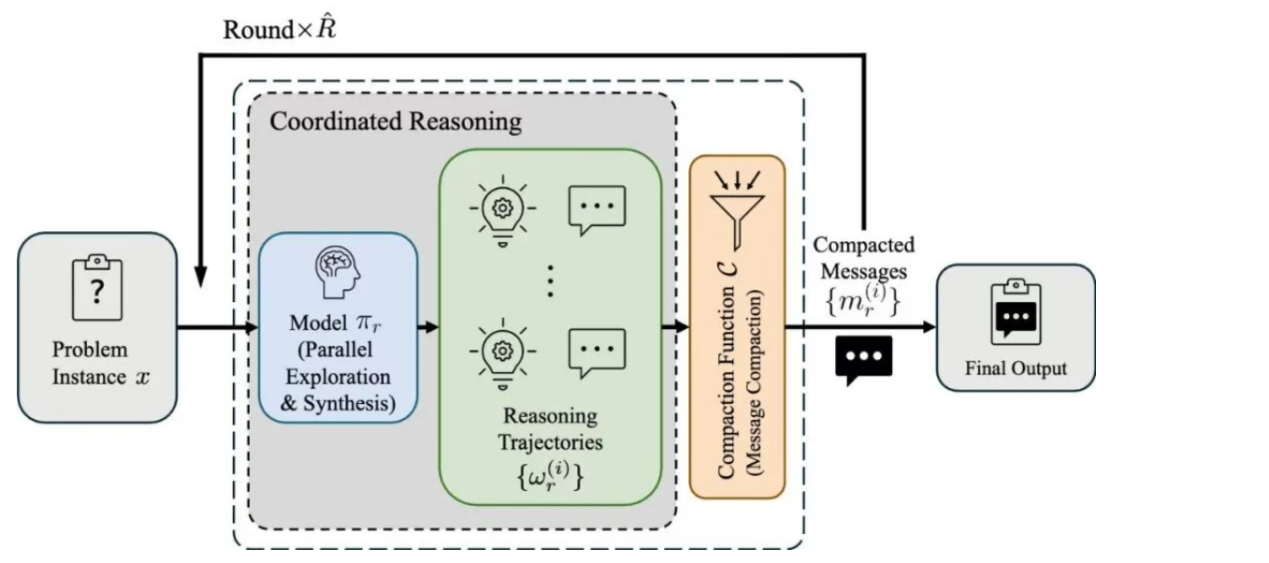
\includegraphics{images/image-0034.png}
\caption{PaCoRe 并行协同推理工作流}
\end{figure}

\hypertarget{ux4e8cux548cux57faux4e8eux641cux7d22ux7684ux65b9ux6cd5ux591aux667aux80fdux4f53ux65b9ux6cd5ux7684ux6bd4ux8f83}{%
\subsubsection{（二）和基于搜索的方法、多智能体方法的比较}\label{ux4e8cux548cux57faux4e8eux641cux7d22ux7684ux65b9ux6cd5ux591aux667aux80fdux4f53ux65b9ux6cd5ux7684ux6bd4ux8f83}}

和基于搜索的方法相比：基于搜索的推理是在每一步搜索多种路径、选择最优，以在解空间中寻找一条最优路径；而PaCoRe是并行展开多路推理直到最后，再进行视角的反复碰撞与融合，让模型自己``讨论''出一个收敛的结论。

和多智能体方法相比：多智能体架构中多个Agent往往有不同的System Prompt从而扮演不同角色，或为不同模型，这里只用了一个模型并行输出不同的推理过程，并在下一轮回馈给自身，相当于多个相同的Agent。

\hypertarget{ux4e09ux5173ux4e8eux5e76ux884cux63a8ux7406ux7684ux62d3ux5c55ux63a2ux8ba8}{%
\subsubsection{（三）关于并行推理的拓展探讨}\label{ux4e09ux5173ux4e8eux5e76ux884cux63a8ux7406ux7684ux62d3ux5c55ux63a2ux8ba8}}

除此架构外，其他并行推理架构还提出了一些不同的技术路径。

动态剪枝：在推理过程中，模型自身或一个专门的验证模型会实时评估当前路径的置信度，发现某条路径逻辑不通或概率降低时，自动``剪枝''终止该分支（Pruning），将计算资源集中到更有希望的路径上。但这对验证能力有较高的要求。

动态调整深度：系统会根据问题的复杂度，自动调整 thinking\_level（思考深度）。简单的问候直接回答，复杂的数学题则自动分配更多计算资源进行并行推演。

\hypertarget{ux53c2ux8003ux6587ux732e-126}{%
\subsection{参考文献}\label{ux53c2ux8003ux6587ux732e-126}}

\begin{itemize}
\tightlist
\item
  Zhu, J., Zhang, G., Ma, X., et al.~(2026). \href{https://arxiv.org/abs/2602.02486}{RE-TRAC: REcursive TRAjectory Compression for Deep Search Agents}. arXiv:2602.02486.
\item
  StepFun AI. (2025). \href{https://github.com/stepfun-ai/PaCoRe/blob/main/pacore_report.pdf}{PaCoRe: Parallel Coordinated Reasoning}. Technical report.
\end{itemize}

\clearpage

\hypertarget{ux601dux7ef4ux793eux4f1aux7406ux8bbaux8bbaux6587}{%
\section{思维社会理论（论文）}\label{ux601dux7ef4ux793eux4f1aux7406ux8bbaux8bbaux6587}}

\begin{quote}
本文是论文阅读笔记，内容代表对应论文方法或作者理解，不应直接视为领域共识或工程最佳实践。
\end{quote}

Google的相关研究指出，当前顶尖推理模型的强大推理能力，并非仅仅源于更长的思维链，还可能源于模型内部隐式地模拟了一个``思维社会''（Society of Thought）。模型在推理时，通过模拟不同视角、不同人格和专业背景的``隐形智能体''之间的对话、辩论和协作，从而实现了比单一视角更强的解决问题能力。

\hypertarget{ux4e00ux5177ux4f53ux8868ux73b0}{%
\subsection{一、具体表现}\label{ux4e00ux5177ux4f53ux8868ux73b0}}

\begin{enumerate}
\def\labelenumi{\arabic{enumi}.}
\item
  对话行为：推理模型频繁出现``提问-回答''、``视角切换''、``观点冲突''和``和解''等对话行为。相比之下，普通模型通常是平铺直叙的单向输出。利用Bales的交互过程分析（IPA），研究发现推理模型的对话行为不仅有信息交换，还包含``社会情感角色''的互动，例如表达反对或达成一致，这种互动随着问题难度的增加而变得更加频繁。
\item
  ``人格''与``专长''多样性：推理轨迹中包含多种隐式声音，这些声音在人格测试中表现出显著差异；模型也调用了不同领域的``专家''视角进行互动，避免了单一视角的偏见，促进了对解决方案空间的更有效探索。
\end{enumerate}

\hypertarget{ux4e8cux63a8ux7406ux80fdux529bux63d0ux5347ux7684ux76f8ux5173ux53d1ux73b0}{%
\subsection{二、推理能力提升的相关发现}\label{ux4e8cux63a8ux7406ux80fdux529bux63d0ux5347ux7684ux76f8ux5173ux53d1ux73b0}}

\begin{enumerate}
\def\labelenumi{\arabic{enumi}.}
\item
  激活``对话特征''能提升推理能力。如在模型中找到并增强了一个代表``对话中的惊讶/转折''（类似 ``Oh!'', ``Wait\ldots{}''）的特征，增强这一个对话特征，模型的数学推理准确率就大大提高，这证明了对话式的交互结构与推理能力之间存在因果关系。
\item
  即使只奖励最终答案的正确性（不奖励对话格式），模型在RL训练过程中也会自发地演化出提问、反思等对话行为。
\item
  训练方法启示：如果预先用``多智能体对话''数据对模型进行微调（SFT），再进行强化学习，模型的学习速度和最终性能都显著优于用``独白式思维链''微调的模型。这表明对话结构本身就是一种高效的推理脚手架。
\end{enumerate}

\hypertarget{ux53c2ux8003ux6587ux732e-127}{%
\subsection{参考文献}\label{ux53c2ux8003ux6587ux732e-127}}

\begin{itemize}
\tightlist
\item
  Du, Y., Li, S., Torralba, A., Tenenbaum, J. B., \& Mordatch, I. (2023). \href{https://arxiv.org/abs/2305.14325}{Improving Factuality and Reasoning in Language Models through Multiagent Debate}. arXiv:2305.14325.
\item
  Kim, J., Lai, S., Scherrer, N., Agüera y Arcas, B., \& Evans, J. (2026). \href{https://arxiv.org/abs/2601.10825}{Reasoning Models Generate Societies of Thought}. arXiv:2601.10825.
\end{itemize}

\clearpage
